%%%%%%%%%%%%%%%%%%%%%%%%%%%%%%%%%%%%%%%%%
% Beamer Presentation
% LaTeX Template
% Version 1.0 (10/11/12)
%
% This template has been downloaded from:
% http://www.LaTeXTemplates.com
%
% License:
% CC BY-NC-SA 3.0 (http://creativecommons.org/licenses/by-nc-sa/3.0/)
%
%%%%%%%%%%%%%%%%%%%%%%%%%%%%%%%%%%%%%%%%%

%----------------------------------------------------------------------------------------
%	PACKAGES AND THEMES
%----------------------------------------------------------------------------------------

\documentclass{beamer}

\mode<presentation> {

% The Beamer class comes with a number of default slide themes
% which change the colors and layouts of slides. Below this is a list
% of all the themes, uncomment each in turn to see what they look like.

%\usetheme{default}
%\usetheme{AnnArbor}
%\usetheme{Antibes}
%\usetheme{Bergen}
%\usetheme{Berkeley}
%\usetheme{Berlin}
%\usetheme{Boadilla}
%\usetheme{CambridgeUS}
%\usetheme{Copenhagen}
\usetheme{Darmstadt}
%\usetheme{Dresden}
%\usetheme{Frankfurt}
%\usetheme{Goettingen}
%\usetheme{Hannover}
%\usetheme{Ilmenau}
%\usetheme{JuanLesPins}
%\usetheme{Luebeck}
%\usetheme{Madrid}
%*\usetheme{Malmoe}
%\usetheme{Marburg}
%\usetheme{Montpellier}
%\usetheme{PaloAlto}
%\usetheme{Pittsburgh}
%\usetheme{Rochester}
%\usetheme{Singapore}
%\usetheme{Szeged}
%\usetheme{Warsaw}

% As well as themes, the Beamer class has a number of color themes
% for any slide theme. Uncomment each of these in turn to see how it
% changes the colors of your current slide theme.

%\usecolortheme{albatross}
%\usecolortheme{beaver}
%\usecolortheme{beetle}
%\usecolortheme{crane}
%\usecolortheme{dolphin}
%\usecolortheme{dove}
%\usecolortheme{fly}
%\usecolortheme{lily}
\usecolortheme{orchid}
%\usecolortheme{rose}
%\usecolortheme{seagull}
%\usecolortheme{seahorse}
%\usecolortheme{whale}
%\usecolortheme{wolverine}

%\setbeamertemplate{footline} % To remove the footer line in all slides uncomment this line
%\setbeamertemplate{footline}[page number] % To replace the footer line in all slides with a simple slide count uncomment this line

%\setbeamertemplate{navigation symbols}{} % To remove the navigation symbols from the bottom of all slides uncomment this line
}


\usepackage{graphicx} % Allows including images
\usepackage{booktabs} % Allows the use of \toprule, \midrule and \bottomrule in tables
\usepackage{xspace}
\usepackage{caption}
\usepackage{subfigure}
\usepackage[english,brazil]{babel}
\usepackage[utf8]{inputenc}

%Renomeia o nome padrao das figuras.
\renewcommand{\figurename}{Figura}
\renewcommand{\tablename}{Tabela}
%----------------------------------------------------------------------------------------
%	TITLE PAGE
%----------------------------------------------------------------------------------------

\title[Computação Gráfica]{Visualização} % The short title appears at the bottom of every slide, the full title is only on the title page

\author{Uéliton Freitas} % Your name
\institute[UFMS] % Your institution as it will appear on the bottom of every slide, may be shorthand to save space
{
Universidade Católica Don Bosco - UCDB \\ % Your institution for the title page
\medskip
\textit{freitas.ueliton@gmail.com} % Your email address
}
\date{\today} % Date, can be changed to a custom date


\begin{document}

\begin{frame}
\titlepage % Print the title page as the first slide
\end{frame}

\begin{frame}
\frametitle{Sumário} % Table of contents slide, comment this block out to remove it
\tableofcontents % Throughout your presentation, if you choose to use \section{} and \subsection{} commands, these will automatically be printed on this slide as an overview of your presentation
\end{frame}




%----------------------------------------------------------------------------------------
%	PRESENTATION SLIDES
%----------------------------------------------------------------------------------------

%------------------------------------------------
\section{Introdução} 
%------------------------------------------------

%\section{Speeded-Up Robust Features - SURF} % A subsection can be created just before a set of slides with a common theme to further break down your presentation into chunks
%\section{Baf Of Features and Colors}

%\section{Refer\^encias}
%%%%%%%%%%%%%%%%%%%%%%%%%%%%%%%%%%%%%%%%%%%%%%%%%%%%%%%%%%%%%%%%%%%%%%%%%%%%%%%%%%%%%%%%%%
\begin{frame}
\frametitle{Introdução}


	\begin{block}{Visualização}
		\begin{itemize}
			\item<1-> Determina quais partes serão mostradas na tela.
			\item<2-> A imagem é determinada no \textbf{Sistema de Coordenadas do Mundo (World Coordinates)}, cujas partes selecionadas são mostradas no \textbf{Sistema de Coordenadas Locais (Local Coordinates)}.
			\begin{itemize}
				\item Este processo envolve várias transformações: Rotação, Translações...
				\item Operações para eliminar partes da imagem que estão fora da imagem de exibição.	
			\end{itemize}			 
		\end{itemize}
	\end{block}
	
\end{frame}



%%%%%%%%%%%%%%%%%%%%%%%%%%%%%%%%%%%%%%%%%%%%%%%%%%%%%%%%%%%%%%%%%%%%%%%%%%%%%%%%%%%%%%%%%%
\begin{frame}
\frametitle{Introdução}


	\begin{block}{Janela de Recorte ou Clipping Window}
		\begin{itemize}
			\item Uma secção da cena é selecionada.
			\item O que estiver fora da cena não será mostrado.
		\end{itemize}
	\end{block}
	
	\begin{block}{View Port}
		\begin{itemize}
			\item A janela de recorte pode ser posicionada dentro de uma outra janela de recorte denominada \textbf{Viewport}.
			\begin{itemize}
				\item Objetos dentro da \textbf{Janela de Recorte}(o que será visto) são posicionados dentro de uma \textbf{Viewport}, que por usa vez posiciona os objetos dentro da janela de sistema (onde serão visto).
				\item \textbf{Multiplas Viewports} podem ser utilizadas para mostrar várias partes de uma cena.
			\end{itemize}
		\end{itemize}
	\end{block}
	
\end{frame}







%%%%%%%%%%%%%%%%%%%%%%%%%%%%%%%%%%%%%%%%%%%%%%%%%%%%%%%%%%%%%%%%%%%%%%%%%%%%%%%%%%%%%%%%%%
\begin{frame}
\frametitle{Introdução}

	\begin{figure}[!h]
			\begin{center}
			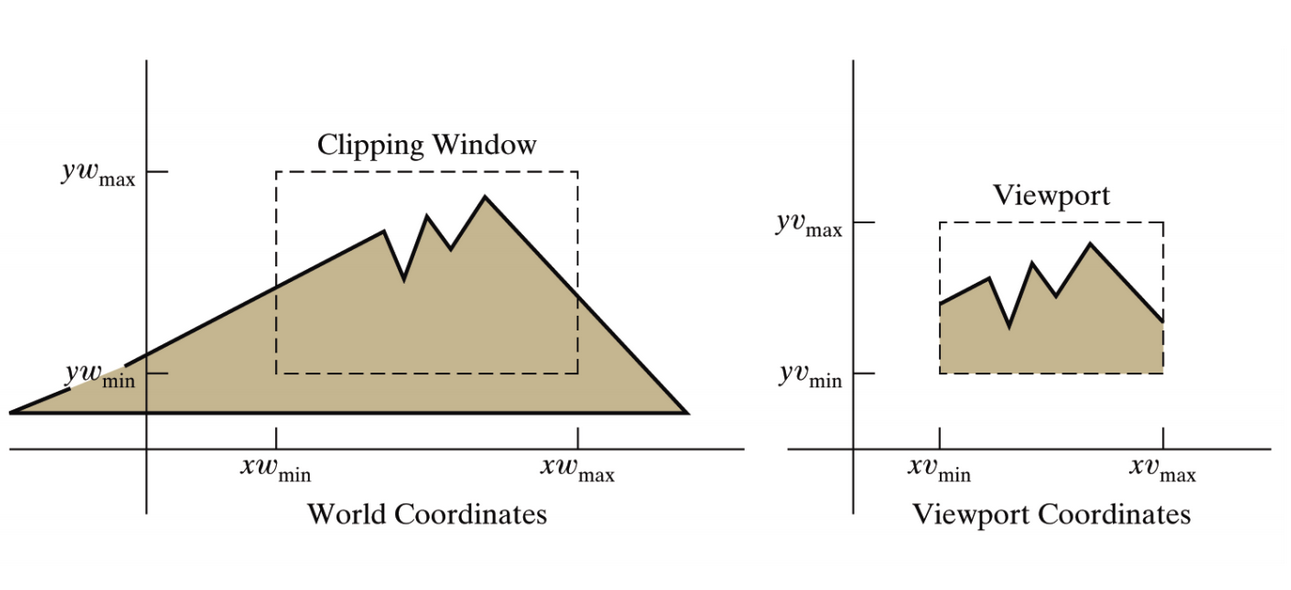
\includegraphics[width=0.9\textwidth]{Figures/CliWin}
			\end{center}
	\end{figure}	
\end{frame}


%%%%%%%%%%%%%%%%%%%%%%%%%%%%%%%%%%%%%%%%%%%%%%%%%%%%%%%%%%%%%%%%%%%%%%%%%%%%%%%%%%%%%%%%%%
\begin{frame}
\frametitle{Introdução}

	\begin{block}{Transformação da Visão}
		\begin{itemize}
			\item Mapeamento do sistema de coordenadas do sistema de coordenadas mundo para o sistema de coordenadas de dispositivo.

			\item As coordenadas dos objetos são \textbf{normalizadas} entre 0 e 1 para acelerar o processo de recorte.
		\end{itemize}
		
	\end{block}
	\begin{figure}[!h]
				\begin{center}
					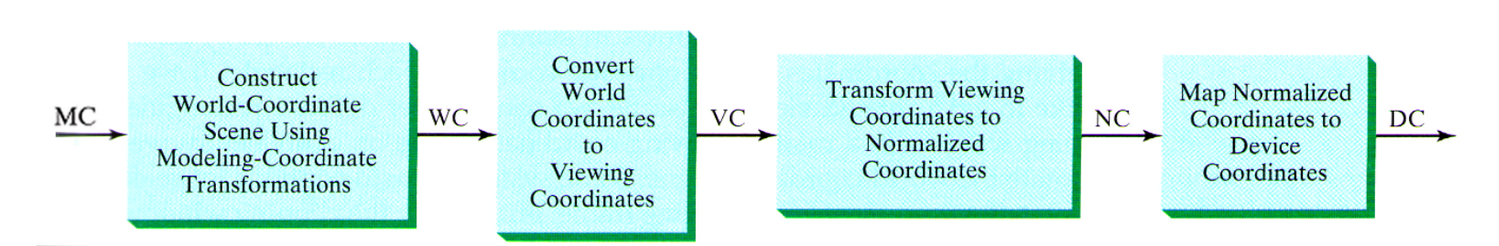
\includegraphics[width=0.9\textwidth]{Figures/ViePip}
				\end{center}
			\end{figure}	
\end{frame}

%%%%%%%%%%%%%%%%%%%%%%%%%%%%%%%%%%%%%%%%%%%%%%%%%%%%%%%%%%%%%%%%%%%%%%%%%%%%%%%%%%%%%%%%%%
\section{Janela De Recorte}
\begin{frame}
\frametitle{Janela de Recorte}

	\begin{block}{Janela de Recorte}
		\begin{itemize}
			\item Devido ao custo computacional as API's gráficas criam \textbf{Janelas de Recorte} em formato retangular com eixos $x$ e $y$. 
			\item Geralmente a \textbf{Janela de Recorte} é definida no sistema de coordenadas do mundo.
			\item Geralmente, a transformação de visão é definida em um sistema de coordenadas de visão dentro do sistema de coordenadas mundo.
				\begin{itemize}
					\item Assim é possível determinar uma janela retangular em qualquer orientação.
					\item Uma visão das coordenadas do mundo é obtida transformando a cena para as coordenadas de visão.
				\end{itemize}				 
		\end{itemize}
		
	\end{block}


\end{frame}

%%%%%%%%%%%%%%%%%%%%%%%%%%%%%%%%%%%%%%%%%%%%%%%%%%%%%%%%%%%%%%%%%%%%%%%%%%%%%%%%%%%%%%%%%%
\begin{frame}
\frametitle{Janela de Recorte}

	\begin{figure}[!h]
				\begin{center}
					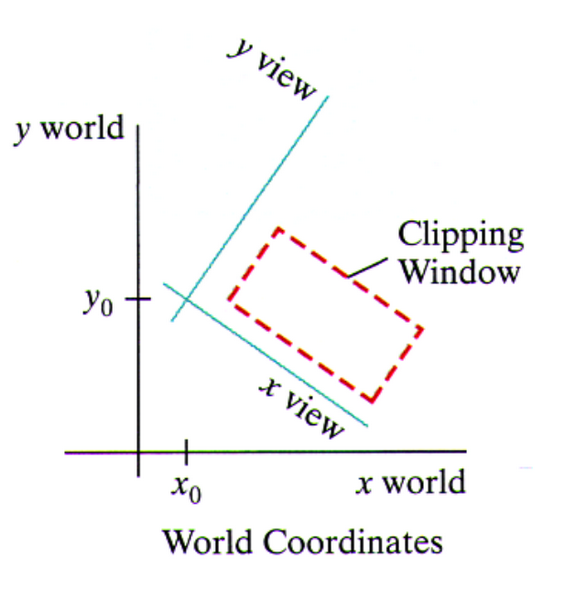
\includegraphics[width=0.6\textwidth]{Figures/janRec}
				\end{center}
			\end{figure}	
\end{frame}
%%%%%%%%%%%%%%%%%%%%%%%%%%%%%%%%%%%%%%%%%%%%%%%%%%%%%%%%%%%%%%%%%%%%%%%%%%%%%%%%%%%%%%%%%%
\begin{frame}
\frametitle{Janela de Recorte}

	\begin{block}{Sistema De Coordenada da Janela de Recorte}
		\begin{itemize}
			\item<1->	Escolhe-se um ponto $\textbf{P}_0 = (x_0,y_0)$ no sistema de coordenadas de visão e uma orientação obtida por meio de um vetor $\textbf{V}$ que orienta o eixo $y_{view}$.  
			\begin{itemize}
				\item \textbf{V} é chamado de \textbf{view-up vector}.
			\end{itemize}
			\item<2-> Com o sistema de coordenadas de visão definido, são utilizadas translações e rotações para transformar as diferentes descrições de objetos para sobrepor os diferentes sistemas de coordenadas.
			\begin{enumerate}
				\item Translada-se $\textbf{P}_0$ para a origem do sistema de coordenadas do mundo.
				\item O sistema é rotacionado para coincidir com o sistema de coordenadas do mundo.
			\end{enumerate}	
			\item<3-> A conversão é dada por:\\
				\begin{equation*}
					\textbf{M}_{WC,VC} = \textbf{R} \cdot \textbf{T}
				\end{equation*}						 
		\end{itemize}
		
	\end{block}
\end{frame}


%%%%%%%%%%%%%%%%%%%%%%%%%%%%%%%%%%%%%%%%%%%%%%%%%%%%%%%%%%%%%%%%%%%%%%%%%%%%%%%%%%%%%%%%%%
\begin{frame}
\frametitle{Janela de Recorte}

	\begin{figure}[!h]
				\begin{center}
					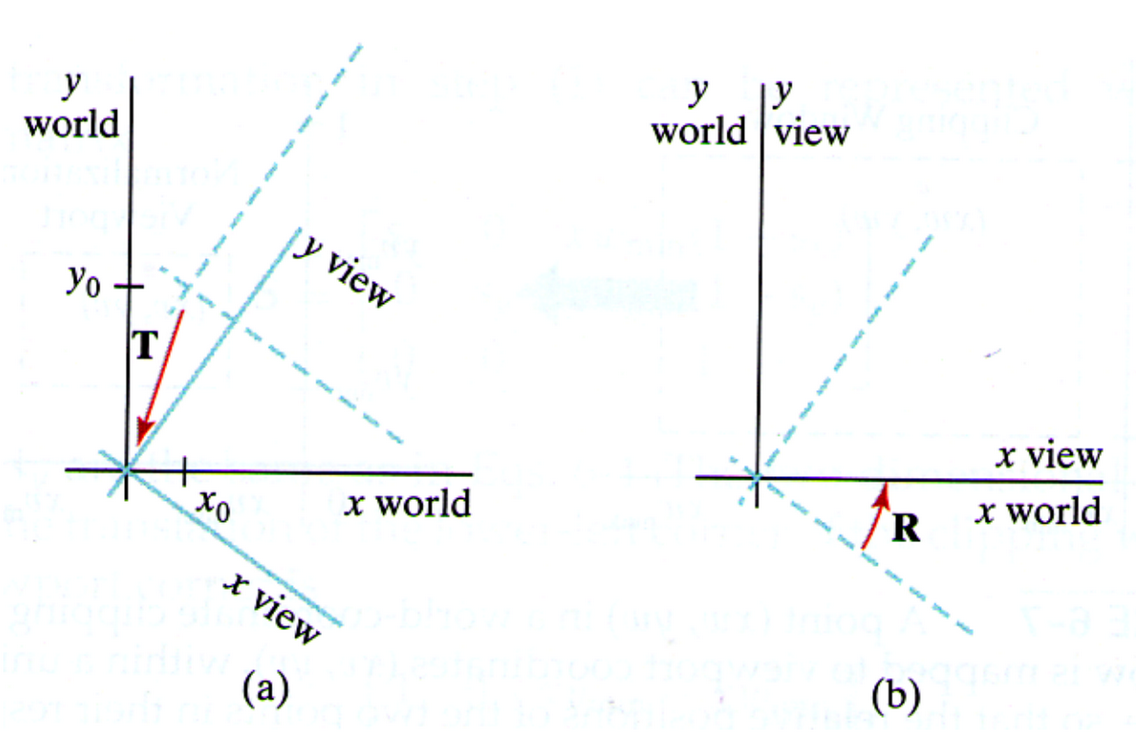
\includegraphics[width=0.8\textwidth]{Figures/WcVc}
				\end{center}
			\end{figure}	
\end{frame}

%%%%%%%%%%%%%%%%%%%%%%%%%%%%%%%%%%%%%%%%%%%%%%%%%%%%%%%%%%%%%%%%%%%%%%%%%%%%%%%%%%%%%%%%%%
\begin{frame}
\frametitle{Normalizações e Transformações }

	\begin{block}{Normalizações e Transformações da Viewport}
		\begin{itemize}
			\item Em alguns sistemas as normalizações e transformações da \textbf{Window-Viewport} são feitas em uma mesma operação.
			\begin{itemize}
				\item As coordenadas da viewport são definidas entre 0 e 1.
				\item O quadrado unitário formado é então mapeado para o sistema de saída.
			\end{itemize}
			
			\item Em outros sistemas, as normalizações e transformações são aplicadas antes das transformações da viewport.
			\begin{itemize}
				\item Neste caso, as coordenadas da viewport são as coordenadas da tela.
			\end{itemize}					 
		\end{itemize}
		
	\end{block}
\end{frame}

%%%%%%%%%%%%%%%%%%%%%%%%%%%%%%%%%%%%%%%%%%%%%%%%%%%%%%%%%%%%%%%%%%%%%%%%%%%%%%%%%%%%%%%%%%
\begin{frame}
\frametitle{Normalizações e Transformações }

	\begin{block}{Mapeando uma Janela de Recorte para uma Viewport Normalizada}
		\begin{itemize}
			\item Considerando uma viewport normalizada com valores entre 0 e 1, é necessário mapear a descrição de um objeto de modo que a sua posição seja mantida de acordo com a \textbf{janela de recorte}. 	 
		\end{itemize}	
	\end{block}
	
	\begin{figure}[!h]
			\begin{center}
				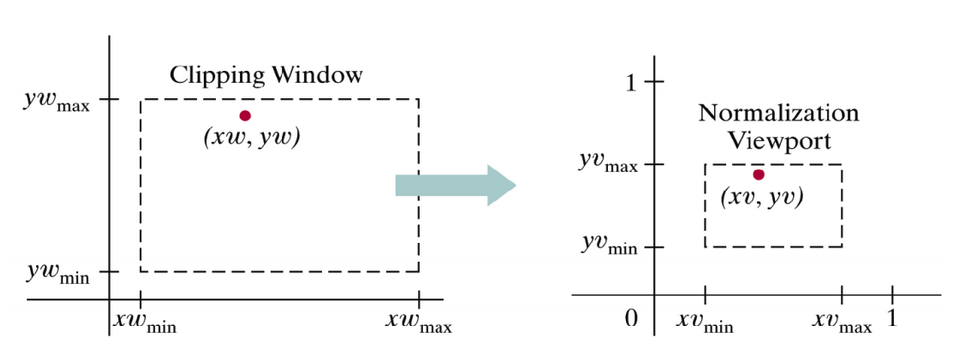
\includegraphics[width=0.8\textwidth]{Figures/VieNor}
			\end{center}
	\end{figure}	
\end{frame}

%%%%%%%%%%%%%%%%%%%%%%%%%%%%%%%%%%%%%%%%%%%%%%%%%%%%%%%%%%%%%%%%%%%%%%%%%%%%%%%%%%%%%%%%%%
\begin{frame}
\frametitle{Normalizações e Transformações }

	\begin{block}{Mapeando uma Janela de Recorte para uma Viewport Normalizada}
		\begin{itemize}
			\item Para transformar um ponto no sistema de coordenadas do mundo para a viewport é necessário:
			\begin{eqnarray*}
				\frac{xv-xv_{min}}{xv_{max}-xv_{min}} = \frac{xw-xw_{min}}{xw_{max}-xw_{min}}\\
				\frac{yv-yv_{min}}{yv_{max}-yv_{min}} = \frac{yw-yw_{min}}{yw_{max}-yw_{min}}
			\end{eqnarray*}	
			
		\item Para as posições $xv$ e $yv$ temos:
			\begin{eqnarray*}
				xv = S_x \cdot xw + t_x \\
				yv = S_y \cdot yw + t_y
			\end{eqnarray*}					 	 
		\end{itemize}	
	\end{block}
	
\end{frame}


%%%%%%%%%%%%%%%%%%%%%%%%%%%%%%%%%%%%%%%%%%%%%%%%%%%%%%%%%%%%%%%%%%%%%%%%%%%%%%%%%%%%%%%%%%
\begin{frame}
\frametitle{Normalizações e Transformações }

	\begin{block}{Mapeando uma Janela de Recorte para uma Viewport Normalizada}
		\begin{itemize}
			\item Os fatores de escala são:
				\begin{eqnarray*}
					S_x = \frac{xv_{max} - xv_{min}}{xw_{max} - xw_{min}} \\
					S_y = \frac{yv_{max} - yv_{min}}{yw_{max} - yw_{min}}
				\end{eqnarray*}
				
			\item Como fatores de translação temos:
				\begin{eqnarray*}
					t_x = \frac{xw_{max} \cdot xv_{min} - xw_{min} \cdot xv_{max}}{xw_{max} - xw_{min}} \\
					t_y = \frac{yw_{max} \cdot yv_{min} - yw_{min} \cdot yv_{max}}{yw_{max} - yw_{min}}
				\end{eqnarray*}		 	 
		\end{itemize}	
	\end{block}
	
\end{frame}

%%%%%%%%%%%%%%%%%%%%%%%%%%%%%%%%%%%%%%%%%%%%%%%%%%%%%%%%%%%%%%%%%%%%%%%%%%%%%%%%%%%%%%%%%%
\begin{frame}
\frametitle{Normalizações e Transformações }

	\begin{block}{Mapeando uma Janela de Recorte para uma Viewport Normalizada}
		\begin{itemize}
			\item Também é possível mapear o sistema de coordenadas do mundo para a viewport utilizando simples transformações.
				\begin{itemize}
					\item Basta converter o retângulo da janela de recorte na viewport.
					\begin{enumerate}
					\item Escala a janela de recorte para ter o tamanho da viewport usando o ponto fixo $xw_{min}$ e $yw_{min}$.
					\item Translada $xw_{min}$ e $yw_{min}$ para $xv_{min}$ e $yv_{min}$
				\end{enumerate}				
				\end{itemize}
													 	 
		\end{itemize}	
	\end{block}
	
\end{frame}

%%%%%%%%%%%%%%%%%%%%%%%%%%%%%%%%%%%%%%%%%%%%%%%%%%%%%%%%%%%%%%%%%%%%%%%%%%%%%%%%%%%%%%%%%%
\begin{frame}
\frametitle{Normalizações e Transformações }

	\begin{block}{Mapeando uma Janela de Recorte para uma Viewport Normalizada}
		\begin{itemize}
			\item Termos como matriz de escala\\
			\begin{equation*}
				\textbf{S} = \begin{bmatrix}
					s_x	&	0	&	xw_{min}(1-s_x) \\
					0	&	s_y	&	yw_{min}(1-s_y) \\
					0	&	0	&	1
				\end{bmatrix}
			\end{equation*}
			
			\item E a matriz de translação como sendo\\
			\begin{equation*}
				\textbf{T} = \begin{bmatrix}
					1	&	0	&	xv_{min} - xw_{min} \\
					0	&	1	&	yv_{min} - yw_{min} \\
					0	&	0	&	1
				\end{bmatrix}
			\end{equation*}			 
		\end{itemize}	
	\end{block}
\end{frame}


%%%%%%%%%%%%%%%%%%%%%%%%%%%%%%%%%%%%%%%%%%%%%%%%%%%%%%%%%%%%%%%%%%%%%%%%%%%%%%%%%%%%%%%%%%
\begin{frame}
\frametitle{Normalizações e Transformações }

	\begin{block}{Mapeando uma Janela de Recorte para uma Viewport Normalizada}
		\begin{itemize}
			\item Termos como matriz composta
			\begin{equation*}
				\textbf{M}_{window,normview} = \textbf{S} \cdot \textbf{T}
			\end{equation*}
			
			\item como sendo\\
			\begin{equation*}
				\textbf{M}_{window,normview} = \begin{bmatrix}
					s_x	&	0	&	t_x \\
					0	&	s_y	&	t_y \\
					0	&	0	&	1
				\end{bmatrix}
			\end{equation*}	
			\item com $s_x,s_y,t_x$ e $t_y$ dados anteriormente.		 
		\end{itemize}	
	\end{block}
\end{frame}

%%%%%%%%%%%%%%%%%%%%%%%%%%%%%%%%%%%%%%%%%%%%%%%%%%%%%%%%%%%%%%%%%%%%%%%%%%%%%%%%%%%%%%%%%%
\begin{frame}
\frametitle{Normalizações e Transformações }

	\begin{block}{Mapeando uma Janela de Recorte para uma Viewport Normalizada}
		\begin{itemize}
			\item Neste mapeamento as posições relativas de cada objeto são mantidas.
				\begin{itemize}
					\item Se um objeto aparece na janela de recorte o mesmo aparece na viewport.
				\end{itemize}
			\item A proporção do objeto será mantida somente se a razão do aspecto da janela de recorte for a mesma da viewport.
				\begin{itemize}
					\item Ou seja, $s_x = s_y$.
				\end{itemize}							 
		\end{itemize}	
	\end{block}
\end{frame}

%%%%%%%%%%%%%%%%%%%%%%%%%%%%%%%%%%%%%%%%%%%%%%%%%%%%%%%%%%%%%%%%%%%%%%%%%%%%%%%%%%%%%%%%%%
\begin{frame}
\frametitle{Normalizações e Transformações }

	\begin{block}{Mapeando uma Janela de Recorte para um quadrado normalizado}
		\begin{itemize}
			\item Uma outra abordagem, é transformar a janela de recorte em um quadrado normalizado, fazer os recortes da cena normalizada e então enviar para a viewport com sistema de coordenadas da tela.
			\item Nesta representação os objetos que não estão na cena (fora dos limites $x=\pm1$ e $y=\pm1$) são facilmente removidos da viewport.				 
		\end{itemize}	
	\end{block}
	
	\begin{figure}[!h]
			\begin{center}
				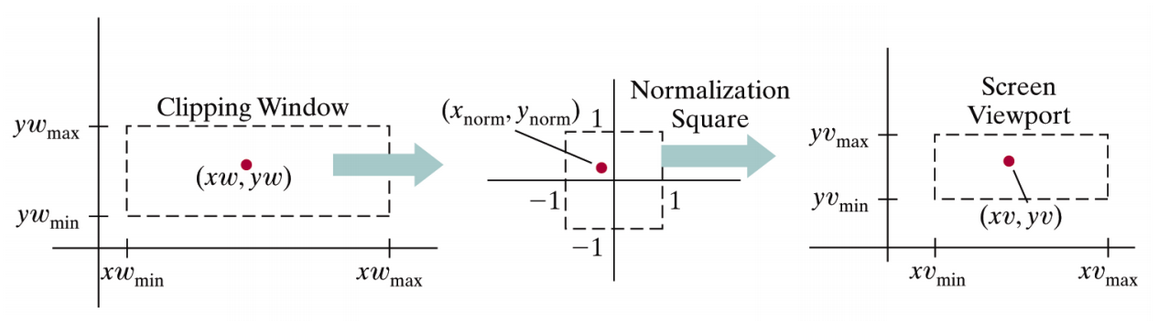
\includegraphics[width=0.8\textwidth]{Figures/QuaNor}
			\end{center}
	\end{figure}	
\end{frame}

%%%%%%%%%%%%%%%%%%%%%%%%%%%%%%%%%%%%%%%%%%%%%%%%%%%%%%%%%%%%%%%%%%%%%%%%%%%%%%%%%%%%%%%%%%
\begin{frame}
\frametitle{Normalizações e Transformações }

	\begin{block}{Mapeando uma Janela de Recorte para um quadrado normalizado}
		\begin{itemize}
			\item Mapeando o conteúdo da janela de recorte para o quadrado normalizado, temos que estabelecer as seguintes coordenadas similarmente ao mapeamento window-viewport fazendo, $x_{v_{min}} = y_{v_{min}} = -1$ e $x_{v_{max}} = y_{v_{max}} = 1$\\
			\end{itemize}	
	\end{block}
	
	\begin{equation*}
				\textbf{M}_{window,normsquare} = \begin{bmatrix}
					\frac{2}{xw_{max}-xw_{min}}	&	0							&	- \frac{xw_{max}+xw_{min}}{xw_{max}-xw_{min}} \\
					0							&	\frac{2}{yw_{max}-yw_{min}}	&	- \frac{yw_{max}+yw_{min}}{yw_{max}-yw_{min}} \\
					0							&	0							&	1
				\end{bmatrix}
			\end{equation*}	
\end{frame}

%%%%%%%%%%%%%%%%%%%%%%%%%%%%%%%%%%%%%%%%%%%%%%%%%%%%%%%%%%%%%%%%%%%%%%%%%%%%%%%%%%%%%%%%%%
\begin{frame}
\frametitle{Normalizações e Transformações }

	\begin{block}{Mapeando uma Janela de Recorte para um quadrado normalizado}
		\begin{itemize}
			\item Após os algoritmos de corte serem aplicados o quadrado de tamanho 2 é então transformado em viewport, $x_{v_{min}} = y_{v_{min}} = 0$ e $x_{v_{max}} = y_{v_{max}} = 1$\\
			\end{itemize}	
	\end{block}
	
	\begin{equation*}
				\textbf{M}_{normsquare,viewport} = \begin{bmatrix}
					\frac{xv_{max}-xv_{min}}{2}	&	0							&	\frac{xv_{max}+xv_{min}}{2} \\
					0							&	\frac{yv_{max}-yv_{min}}{2}	&	\frac{yv_{max}+yv_{min}}{2} \\
					0							&	0							&	1
				\end{bmatrix}
			\end{equation*}	
\end{frame}

%%%%%%%%%%%%%%%%%%%%%%%%%%%%%%%%%%%%%%%%%%%%%%%%%%%%%%%%%%%%%%%%%%%%%%%%%%%%%%%%%%%%%%%%%%
\begin{frame}
\frametitle{Normalizações e Transformações }

	\begin{block}{Mapeando uma Janela de Recorte para um quadrado normalizado}
		\begin{itemize}
			\item Finalmente a viewport é posicionada na tela.
		\end{itemize}
	\end{block}
	
	\begin{figure}[!h]
			\begin{center}
				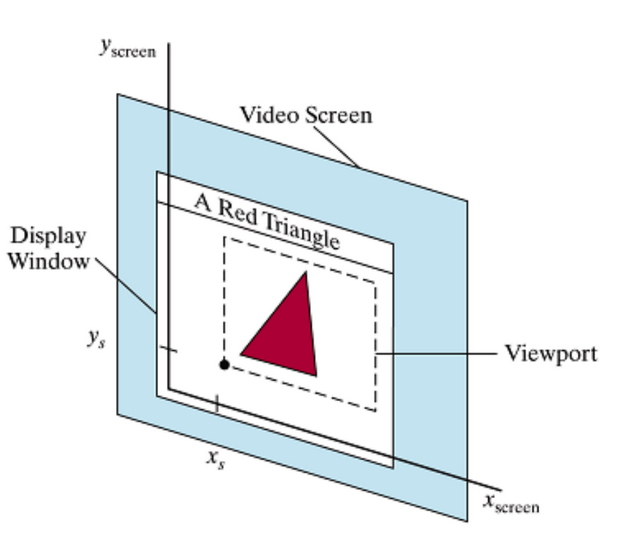
\includegraphics[width=0.6\textwidth]{Figures/QuaNorTel}
			\end{center}
	\end{figure}	
\end{frame}


%%%%%%%%%%%%%%%%%%%%%%%%%%%%%%%%%%%%%%%%%%%%%%%%%%%%%%%%%%%%%%%%%%%%%%%%%%%%%%%%%%%%%%%%%%
\section{Algoritmos de Recorte de Primitivas 2D}
\begin{frame}
\frametitle{Algoritmos de Recorte de Primitivas 2D}

	\begin{block}{Algoritmos de Recorte 2D}
		\begin{itemize}
			\item Define o quais partes dos objetos aparecerão em uma cena.
			\item Identifica quais partes dos objetos estão fora da janela de recorte e elimina a descrição destes objeto no dispositivo de saída.
			\item Por eficiência, os recortes são aplicados nas \textbf{janelas de recorte normalizadas}.
		\end{itemize}
	\end{block}
\end{frame}


%%%%%%%%%%%%%%%%%%%%%%%%%%%%%%%%%%%%%%%%%%%%%%%%%%%%%%%%%%%%%%%%%%%%%%%%%%%%%%%%%%%%%%%%%%
\begin{frame}
\frametitle{Algoritmos de Recorte de Primitivas 2D}

	\begin{block}{Algoritmos de Recorte 2D}
		\begin{itemize}
			\item Existem vários algoritmos para o recorte de:
				\begin{itemize}
					\item Pontos
					\item Linhas
					\item Áreas de Preenchimento(Polígonos).
					\item Curvas
					\item Texto
				\end{itemize}
			\item Os três primeiros são padrões dos pacotes gráficos e apresentam maior rapidez de processamento caso os segmentos sejam retas.
		\end{itemize}
	\end{block}
	

\end{frame}

%%%%%%%%%%%%%%%%%%%%%%%%%%%%%%%%%%%%%%%%%%%%%%%%%%%%%%%%%%%%%%%%%%%%%%%%%%%%%%%%%%%%%%%%%%
\begin{frame}
\frametitle{Algoritmos de Recorte de Primitivas 2D}

	\begin{block}{Algumas Definições}
		\begin{itemize}
			\item Os recortes a seguir serão aplicados em uma janela de recorte retangular na posição padrão com arestas nas fronteiras $xw_{min},xw_{max},yw_{min}$ e $yw_{max}$.
			\item Tipicamente correspondendo ao quadrado normalizado 0 e 1, ou -1 e 1.
		\end{itemize}
	\end{block}
\end{frame}


%%%%%%%%%%%%%%%%%%%%%%%%%%%%%%%%%%%%%%%%%%%%%%%%%%%%%%%%%%%%%%%%%%%%%%%%%%%%%%%%%%%%%%%%%%
\subsection{Recorte de Pontos 2D}
\begin{frame}
\frametitle{Algoritmos de Recorte de Primitivas 2D}

	\begin{block}{Recortes de Pontos 2D}
		\begin{itemize}
			\item Dado um ponto 2D $P=(x,y)$, ele será apresentado no dispositivo de saída se, e somente se:
			\begin{eqnarray*}
				xw_{min}  \leq x \leq xw_{max} \\
				xy_{min}  \leq y \leq yw_{max}
			\end{eqnarray*}
			\item Este processo é útil em recortes de partículas como nuvens, explosões, fumaça, etc.
		\end{itemize}
	\end{block}
\end{frame}

%%%%%%%%%%%%%%%%%%%%%%%%%%%%%%%%%%%%%%%%%%%%%%%%%%%%%%%%%%%%%%%%%%%%%%%%%%%%%%%%%%%%%%%%%%
\subsection{Recorte de Linhas 2D}
\begin{frame}
\frametitle{Algoritmos de Recorte de Primitivas 2D}

	\begin{block}{Recorte de Linhas 2D}
		\begin{itemize}
			\item Processa cada linha de uma utilizando uma série de cálculos e intersecções para definir se a linha, ou parte dela será desenhada.
			\item A tarefa mais cara computacionalmente é o cálculo das intersecções.
		\end{itemize}
	\end{block}
	
	\begin{figure}[!h]
			\begin{center}
				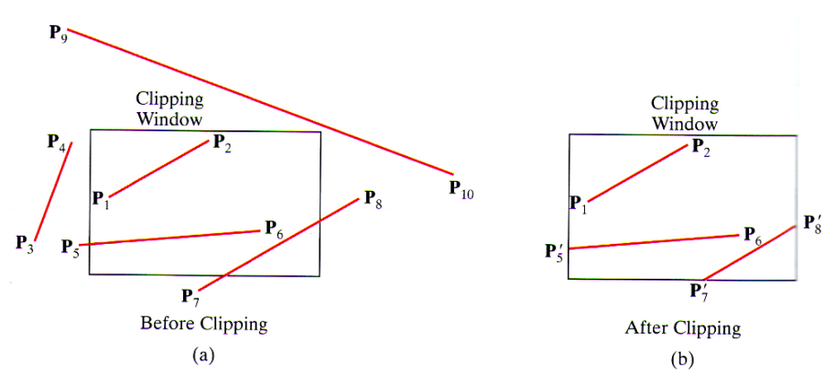
\includegraphics[width=0.6\textwidth]{Figures/LinCli}
			\end{center}
	\end{figure}	
\end{frame}


%%%%%%%%%%%%%%%%%%%%%%%%%%%%%%%%%%%%%%%%%%%%%%%%%%%%%%%%%%%%%%%%%%%%%%%%%%%%%%%%%%%%%%%%%%
\begin{frame}
\frametitle{Algoritmos de Recorte de Primitivas 2D}

	\begin{block}{Recorte de Linhas 2D}
		\begin{itemize}
			\item É fácil determinar se uma linha está completamente dentro da janela. Mas é um pouco mais complicado determinar se a mesma está fora.
			\begin{itemize}
				\item<1-> Quando dois pontos da extremidade de uma linha ($P_1 \: P_2$) estão dentro da janela, então a linha está dentro da janela e será desenhada.
				\item<2-> Quando dois pontos da extremidade de uma linha estão fora de uma das fronteiras da janela (linha $P_3 \: P_4$), a linha está completamente fora.
				\item<3-> Se ambos os testes falham, então a linha intersecta ao menos uma das fronteiras da janela, ou pode não cruzar o interior da mesma. 
			\end{itemize}
		\end{itemize}
	\end{block}
			
\end{frame}


%%%%%%%%%%%%%%%%%%%%%%%%%%%%%%%%%%%%%%%%%%%%%%%%%%%%%%%%%%%%%%%%%%%%%%%%%%%%%%%%%%%%%%%%%%
\begin{frame}
\frametitle{Algoritmos de Recorte de Primitivas 2D}

	\begin{block}{Algoritmos de Recorte de Cohen-Sutherland}
		\begin{itemize}
			\item Um dos primeiros algoritmos para acelerar o processo de recorte.
			\item O tempo de recorte é diminuído executando mais testes antes dos cálculos das intersecções.
		\end{itemize}
	\end{block}
	\begin{block}{Algoritmo de Cohen-Sutherland}
		\begin{itemize}
			\item Inicialmente, cada ponto final de uma linha é assinalado com um \textbf{código de região} constituído de 4 bits.
		\end{itemize}
	\end{block}
	\begin{figure}[!h]
			\begin{center}
				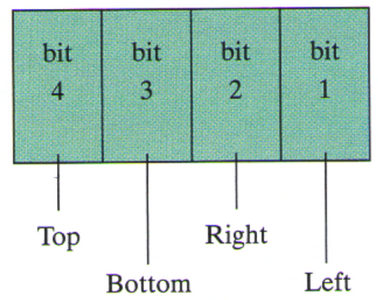
\includegraphics[width=0.3\textwidth]{Figures/Cohen}
			\end{center}
	\end{figure}	
			
\end{frame}

%%%%%%%%%%%%%%%%%%%%%%%%%%%%%%%%%%%%%%%%%%%%%%%%%%%%%%%%%%%%%%%%%%%%%%%%%%%%%%%%%%%%%%%%%%
\begin{frame}
\frametitle{Algoritmos de Recorte de Primitivas 2D}

	\begin{block}{Algoritmos de Recorte de Cohen-Sutherland}
		\begin{itemize}
			\item As quatro fronteiras criam nove regiões de separação no espaço.
			\item Um ponto abaixo e a esquerda da janela recebe os valores 0101 e 000 caso esteja dentro da janela.
		\end{itemize}
	\end{block}
	\begin{figure}[!h]
			\begin{center}
				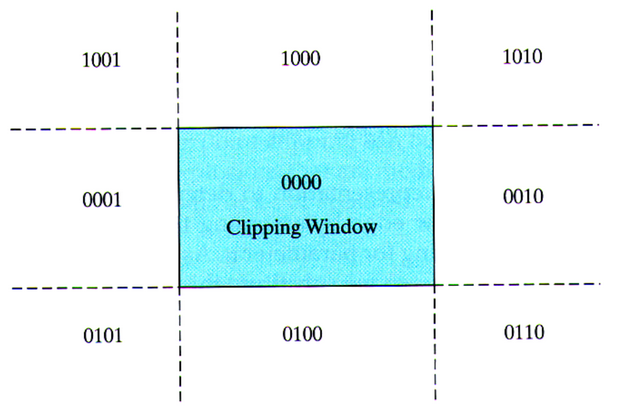
\includegraphics[width=0.6\textwidth]{Figures/FroRec}
			\end{center}
	\end{figure}	
			
\end{frame}

%%%%%%%%%%%%%%%%%%%%%%%%%%%%%%%%%%%%%%%%%%%%%%%%%%%%%%%%%%%%%%%%%%%%%%%%%%%%%%%%%%%%%%%%%%
\begin{frame}
\frametitle{Algoritmos de Recorte de Primitivas 2D}

	\begin{block}{Algoritmos de Recorte de Cohen-Sutherland}
		\begin{itemize}
			\item<1-> Os valores dos bits são obtidos comparando as coordenadas $(x,y)$ com as fronteiras de recortes.
			\begin{itemize}
				\item O bit 1 é definido como 1 caso $x < xw_{min}$.
				\item Os outros bits são obtidos de forma similar.
			\end{itemize}
			\item<2-> É possível fazer esta comparação de forma mais eficiente seguindo dois passos:
				\begin{enumerate}
					\item Calcula-se a diferença entre os pontos e as fronteiras da janela.
					\item Usar o sinal resultante para definir o valor do código (- corresponde a 1, + corresponde a 0).
					\begin{itemize}
						\item bit 1 é o sinal $x-xw_{min}$.
						\item bit 2 é o sinal $xw_{max} - x$.
						\item bit 3 é o sinal $y - yw_{min}$.
						\item bit 3 é o sinal $yw_{max} - y$.
					\end{itemize}
				\end{enumerate}
		\end{itemize}
	\end{block}
\end{frame}

%%%%%%%%%%%%%%%%%%%%%%%%%%%%%%%%%%%%%%%%%%%%%%%%%%%%%%%%%%%%%%%%%%%%%%%%%%%%%%%%%%%%%%%%%%
\begin{frame}
\frametitle{Algoritmos de Recorte de Primitivas 2D}

	\begin{block}{Algoritmos de Recorte de Cohen-Sutherland}
		\begin{itemize}
			\item Assim é possível determinar facilmente se uma linha está totalmente dentro ou fora da janela.
			\begin{itemize}
				\item Linhas totalmente dentro possuem seu pontos com valores 0000.
				\item Linhas com valores 1 na mesma posição estão totalmente fora da janela.
					\begin{itemize}
						\item Uma linha com pontos finais indicando os valores 1001 e 0101 está completamente a esquerda da janela de recorte.
					\end{itemize}
			\end{itemize}
		\end{itemize}
	\end{block}
	
	\begin{figure}[!h]
			\begin{center}
				\subfigure{
					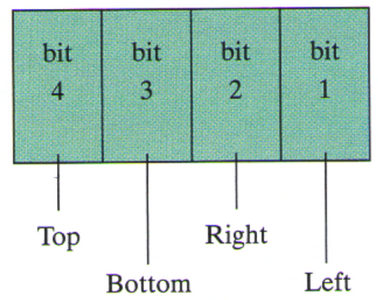
\includegraphics[width=0.3\textwidth]{Figures/Cohen}
				}\qquad
				\subfigure{
					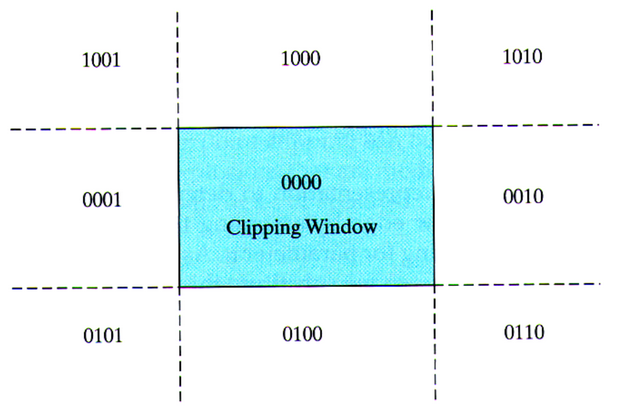
\includegraphics[width=0.3\textwidth]{Figures/FroRec}
				}\qquad
				
			\end{center}
	\end{figure}	
\end{frame}

%%%%%%%%%%%%%%%%%%%%%%%%%%%%%%%%%%%%%%%%%%%%%%%%%%%%%%%%%%%%%%%%%%%%%%%%%%%%%%%%%%%%%%%%%%
\begin{frame}
\frametitle{Algoritmos de Recorte de Primitivas 2D}

	\begin{block}{Algoritmos de Recorte de Cohen-Sutherland}
		\begin{itemize}
			\item Os testes podem ser executados de forma bastante eficiente utilizando operações lógicas simples:
			\begin{itemize}
				\item Quando a operação \textbf{ou} entre os bits for false (0000), a linha está completamente dentro.
				\item Quando a operação \textbf{e} for verdadeira (não 0000) a linha está completamente fora.
			\end{itemize}
		\end{itemize}
	\end{block}
\end{frame}

%%%%%%%%%%%%%%%%%%%%%%%%%%%%%%%%%%%%%%%%%%%%%%%%%%%%%%%%%%%%%%%%%%%%%%%%%%%%%%%%%%%%%%%%%%
\begin{frame}
\frametitle{Algoritmos de Recorte de Primitivas 2D}

	\begin{block}{Algoritmos de Recorte de Cohen-Sutherland}
		\begin{itemize}
			\item As linhas que não há a certeza se estão completamente dentro ou fora da janela são então processadas para ver se há intersecção com a janela.
		\end{itemize}
	\end{block}
	
	\begin{figure}[!h]
			\begin{center}
				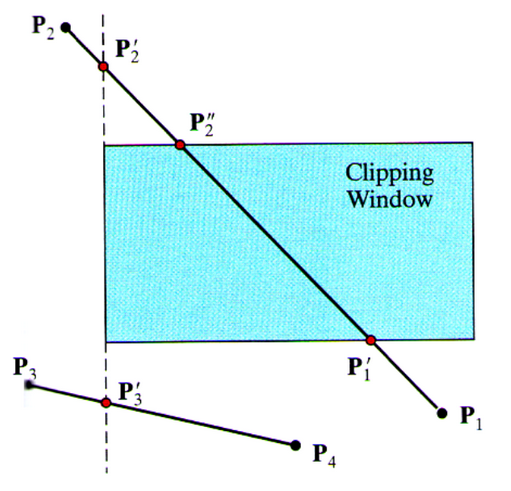
\includegraphics[width=0.4\textwidth]{Figures/IntLin}
			\end{center}
	\end{figure}	
\end{frame}


%%%%%%%%%%%%%%%%%%%%%%%%%%%%%%%%%%%%%%%%%%%%%%%%%%%%%%%%%%%%%%%%%%%%%%%%%%%%%%%%%%%%%%%%%%
\begin{frame}
\frametitle{Algoritmos de Recorte de Primitivas 2D}

	\begin{block}{Algoritmos de Recorte de Cohen-Sutherland}
		\begin{itemize}
			\item<1-> De acordo com a intersecção de cada linha com as fronteiras da janela, a linha é recortada até que sobre apenas o que está dentro da janela, ou nenhuma parte esteja dentro da mesma.
			\item<2-> Para Determinar se a linha cruza a fronteira, basta verificar se o bit da fronteira dos pontos finais variam.
			\begin{itemize}
				\item Se um dos bits for 0 e o outro 1, a linha cruza a fronteira.
			\end{itemize}
		\end{itemize}
	\end{block}
\end{frame}

%%%%%%%%%%%%%%%%%%%%%%%%%%%%%%%%%%%%%%%%%%%%%%%%%%%%%%%%%%%%%%%%%%%%%%%%%%%%%%%%%%%%%%%%%%
\begin{frame}
\frametitle{Algoritmos de Recorte de Primitivas 2D}

	\begin{block}{Verificando a fronteira esquerda}
		\begin{itemize}
			\item $P_1 = 0100$ - Está dentro da fronteira esquerda.
			\item $P_2 = 1001$ - Está fora da fronteira esquerda.
			\begin{itemize}
				\item Calcula a intersecção $P'_2$ e recorta a linha $\overline{P_1P'_2}$
			\end{itemize}
		\end{itemize}
	\end{block}
	
	\begin{figure}[!h]
			\begin{center}
				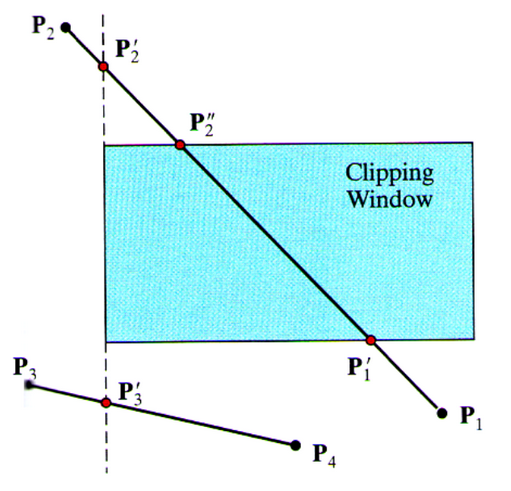
\includegraphics[width=0.4\textwidth]{Figures/IntLin}
			\end{center}
	\end{figure}	
\end{frame}

%%%%%%%%%%%%%%%%%%%%%%%%%%%%%%%%%%%%%%%%%%%%%%%%%%%%%%%%%%%%%%%%%%%%%%%%%%%%%%%%%%%%%%%%%%
\begin{frame}
\frametitle{Algoritmos de Recorte de Primitivas 2D}

	\begin{block}{Intersecção de uma Linha com a Janela}
		\begin{itemize}
			\item Para determinar a intersecção de uma linha com pontos $(x,y)$ e $(x',y')$ podemos usar a equação:
			\begin{eqnarray}
				y' = y + m(x'-x) \\
				x' = x + \frac{y' - y}{m}
			\end{eqnarray}
			\item O valor de $x'$ será $xw_{min}$ ou $xw_{max}$ na Equação 1, e o valor de $y'$ será $yw_{min}$ ou $yw_{max}$ na Equação 2. A inclinação será $m = \frac{y'-y}{x'-x}$
		\end{itemize}
	\end{block}
	
\end{frame}

%%%%%%%%%%%%%%%%%%%%%%%%%%%%%%%%%%%%%%%%%%%%%%%%%%%%%%%%%%%%%%%%%%%%%%%%%%%%%%%%%%%%%%%%%%
\subsection{Recorte de Polígonos 2D}
\begin{frame}
\frametitle{Algoritmos de Recorte de Primitivas 2D}

	\begin{block}{Recorte de Polígonos 2D}
		\begin{itemize}
			\item Para fazer os recortes de polígonos, o algoritmos de recorte de linhas não pode ser utilizado porque, em geral, não gerariam polígonos fechados.
			\begin{itemize}
				\item Produziriam linhas desconexas sem informações de como uni-las.
			\end{itemize}
		\end{itemize}
	\end{block}
	
	\begin{figure}[!h]
			\begin{center}
				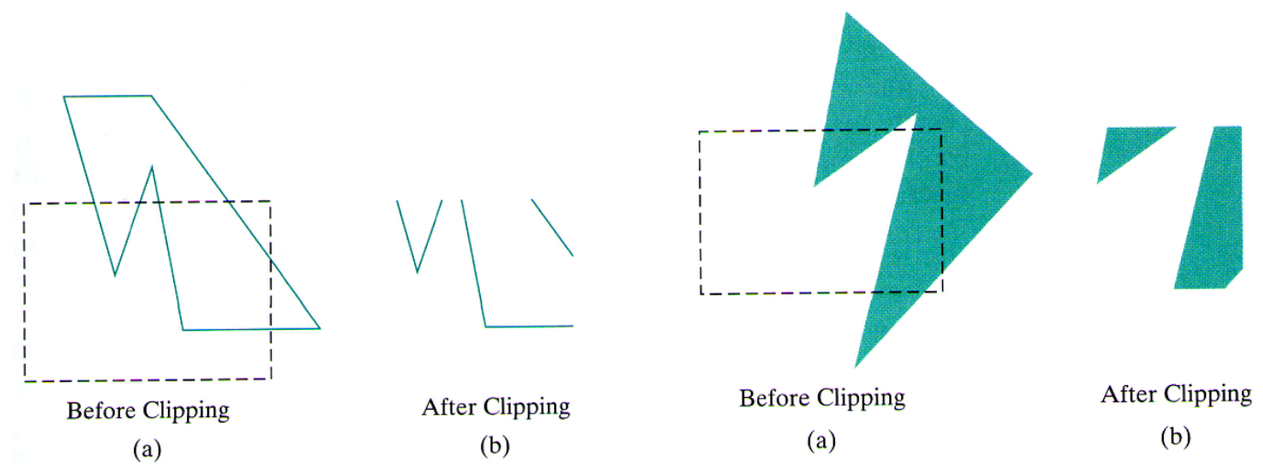
\includegraphics[width=0.7\textwidth]{Figures/RecPol}
			\end{center}
	\end{figure}	
	
\end{frame}


%%%%%%%%%%%%%%%%%%%%%%%%%%%%%%%%%%%%%%%%%%%%%%%%%%%%%%%%%%%%%%%%%%%%%%%%%%%%%%%%%%%%%%%%%%
\begin{frame}
\frametitle{Algoritmos de Recorte de Primitivas 2D}

	\begin{block}{Recorte de Polígonos 2D}
		\begin{itemize}
			\item É possível fazer o recorte de polígonos de forma semelhante ao recorte de linhas.
			\begin{itemize}
				\item Isto é feito formando um novo polígono cada vez que o recorte de uma fronteira é feito.
			\end{itemize}
		\end{itemize}
	\end{block}
	
	\begin{figure}[!h]
			\begin{center}
				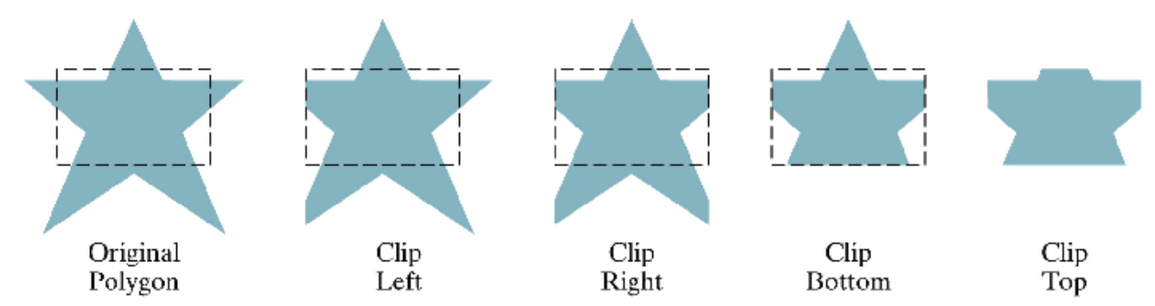
\includegraphics[width=0.8\textwidth]{Figures/RecPol2}
			\end{center}
	\end{figure}	
	
\end{frame}

%%%%%%%%%%%%%%%%%%%%%%%%%%%%%%%%%%%%%%%%%%%%%%%%%%%%%%%%%%%%%%%%%%%%%%%%%%%%%%%%%%%%%%%%%%
\begin{frame}
\frametitle{Algoritmos de Recorte de Primitivas 2D}

	\begin{block}{Recorte de Polígonos 2D}
		\begin{itemize}
			\item Para verificar se um polígono está completamente dentro da janela, basta verificar se suas coordenadas máximas e mínimas estão dentro da janela de recorte.
			\item Quando uma área não pode ser verificada como totalmente dentro da janela, as intersecções são calculadas.
		\end{itemize}
	\end{block}
	
	\begin{figure}[!h]
			\begin{center}
				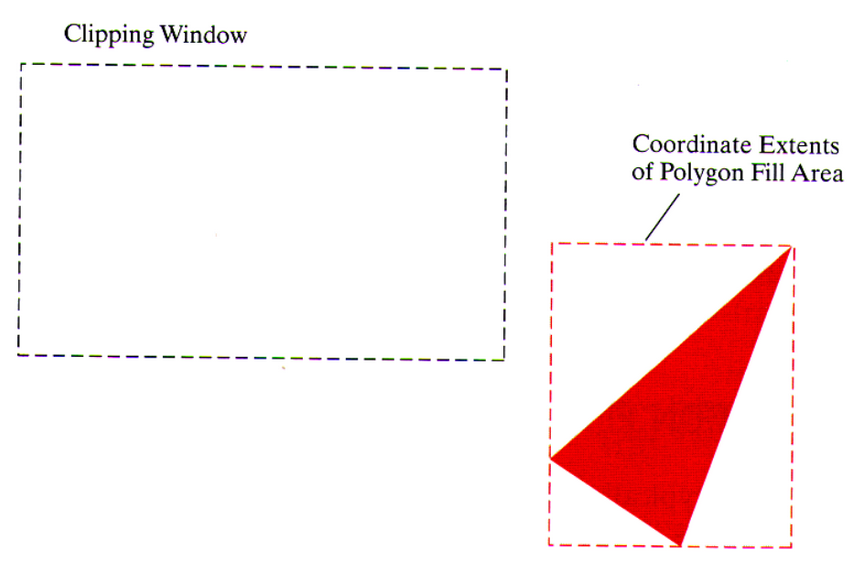
\includegraphics[width=0.5\textwidth]{Figures/RecPolAre}
			\end{center}
	\end{figure}
\end{frame}

%%%%%%%%%%%%%%%%%%%%%%%%%%%%%%%%%%%%%%%%%%%%%%%%%%%%%%%%%%%%%%%%%%%%%%%%%%%%%%%%%%%%%%%%%%
\begin{frame}
\frametitle{Algoritmos de Recorte de Primitivas 2D}

	\begin{block}{Recorte de Polígonos 2D}
		\begin{itemize}
			\item Uma forma simples de ser fazer os recortes é criando uma nova lista de vértices cada vez que são feitos recortes em uma fronteira da janela, e então passar a nova lista de vértices para a nova fronteira.
			\item \textbf{Polígonos Côncavos} podem gerar várias listas de vértices.
		\end{itemize}
	\end{block}
	
	\begin{figure}[!h]
			\begin{center}
				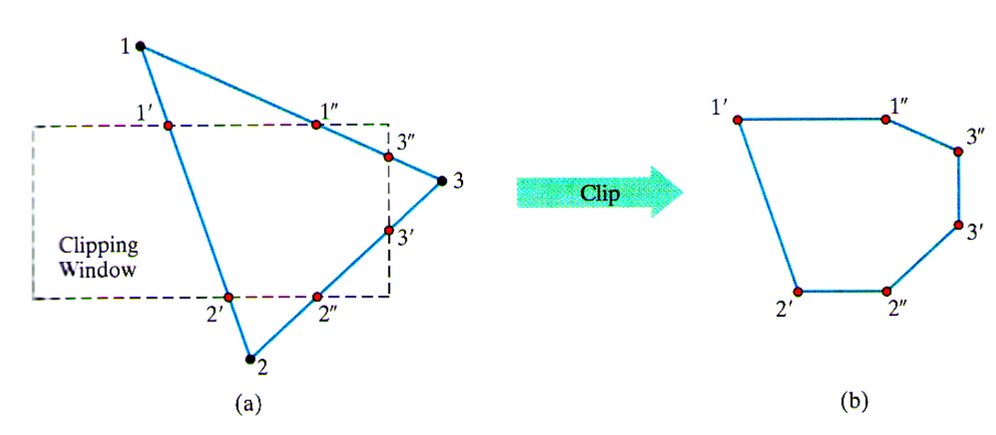
\includegraphics[width=0.7\textwidth]{Figures/RecPolCon}
			\end{center}
	\end{figure}
\end{frame}

%%%%%%%%%%%%%%%%%%%%%%%%%%%%%%%%%%%%%%%%%%%%%%%%%%%%%%%%%%%%%%%%%%%%%%%%%%%%%%%%%%%%%%%%%%
\begin{frame}
\frametitle{Algoritmos de Recorte de Primitivas 2D}

	\begin{block}{Algoritmo de Sutherland-Hodgman}
		\begin{itemize}
			\item Uma forma eficiente de efetuar os recortes é enviar cada vértice do polígono para cada estágio de recorte de forma que os vértices recortados possam ser enviados diretamente para o próximo estágio.
			\begin{itemize}
				\item Elimina a necessidade de uma lista de vértices.
				\item Há possibilidade de efetuar os recortes em paralelo.
			\end{itemize}
		\end{itemize}
	\end{block}
\end{frame}

%%%%%%%%%%%%%%%%%%%%%%%%%%%%%%%%%%%%%%%%%%%%%%%%%%%%%%%%%%%%%%%%%%%%%%%%%%%%%%%%%%%%%%%%%%
\begin{frame}
\frametitle{Algoritmos de Recorte de Primitivas 2D}

	\begin{block}{Algoritmo de Sutherland-Hodgman}
		\begin{itemize}
			\item A principal estratégia deste algoritmos é mandar os pares de pontos finais de cada linha sucessiva do polígono para uma série de recortadores (esquerdo, direito, inferior e superior).
			\item Conforme o recorte é executado para um par de vértice, as coordenadas recortadas são enviadas para o próximo recortador. 
		\end{itemize}
	\end{block}
\end{frame}

%%%%%%%%%%%%%%%%%%%%%%%%%%%%%%%%%%%%%%%%%%%%%%%%%%%%%%%%%%%%%%%%%%%%%%%%%%%%%%%%%%%%%%%%%%
\begin{frame}
\frametitle{Algoritmos de Recorte de Primitivas 2D}

	\begin{block}{Algoritmo de Sutherland-Hodgman}
		\begin{itemize}
			\item Há quatro casos que precisam de atenção nos recortes de arestas de um polígono.
			\begin{enumerate}
				\item	O primeiro ponto final está dentro da janela de recorte e o segundo fora.
				\item	Ambos os pontos finais estão dentro da janela de recorte.
				\item	O primeiro ponto final da aresta está dentro da janela de recorte e o segundo está fora.
				\item Ambos os pontos finais estão fora da janela de recorte.
			\end{enumerate}			 
		\end{itemize}
	\end{block}
\end{frame}

%%%%%%%%%%%%%%%%%%%%%%%%%%%%%%%%%%%%%%%%%%%%%%%%%%%%%%%%%%%%%%%%%%%%%%%%%%%%%%%%%%%%%%%%%%
\begin{frame}
\frametitle{Algoritmos de Recorte de Primitivas 2D}

	\begin{block}{Algoritmo de Sutherland-Hodgman}
		\begin{itemize}
			\item Para facilitar a passagem de um vértice de um recorte para outro, a saída de cada recortador pode ser da seguinte forma:	 
		\end{itemize}
	\end{block}
	\begin{figure}[!h]
			\begin{center}
				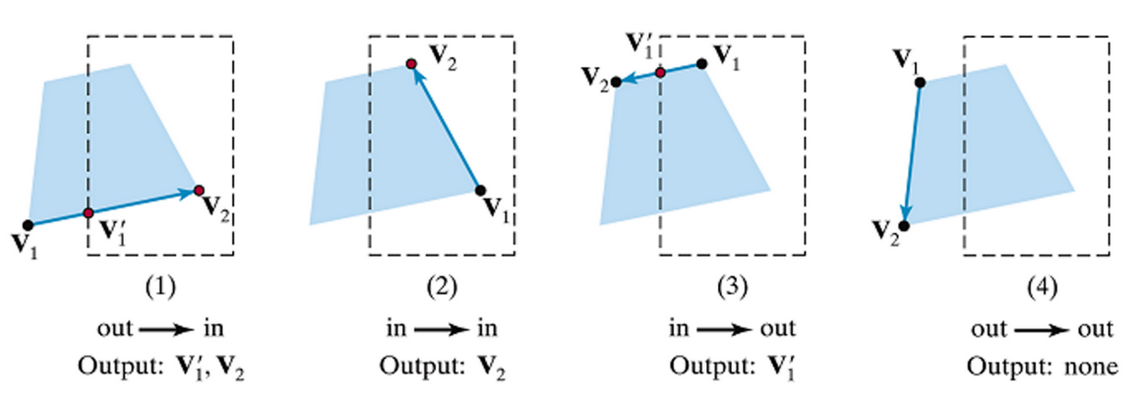
\includegraphics[width=0.7\textwidth]{Figures/RecPol3}
			\end{center}
	\end{figure}
\end{frame}

%%%%%%%%%%%%%%%%%%%%%%%%%%%%%%%%%%%%%%%%%%%%%%%%%%%%%%%%%%%%%%%%%%%%%%%%%%%%%%%%%%%%%%%%%%
\begin{frame}
\frametitle{Algoritmos de Recorte de Primitivas 2D}

	\begin{block}{Algoritmo de Sutherland-Hodgman}
		\begin{itemize}
			\item Conforme cada par de vértice sucessivos é passado para cada um dos recortadores, a saída é gerada de acordo com os seguintes passos:
			\begin{enumerate}
				\item Se o primeiro vértice está fora da janela e o segundo está dentro, a intersecção obtida é enviada juntamente com o segundo vértice para o próximo recorte.
				\item Se ambos os vértices estão dentro, somente o segundo vértice é enviado.
				\item Se o primeiro vértice está dentro da janela e o segundo está fora, é enviado para o próximo recortador somente a intersecção.
				\item Se ambos os vértices estão fora, nada é enviado.
			\end{enumerate}			 
		\end{itemize}
	\end{block}
\end{frame}

%%%%%%%%%%%%%%%%%%%%%%%%%%%%%%%%%%%%%%%%%%%%%%%%%%%%%%%%%%%%%%%%%%%%%%%%%%%%%%%%%%%%%%%%%%
\begin{frame}
\frametitle{Algoritmos de Recorte de Primitivas 2D}

	\begin{figure}[!h]
			\begin{center}
				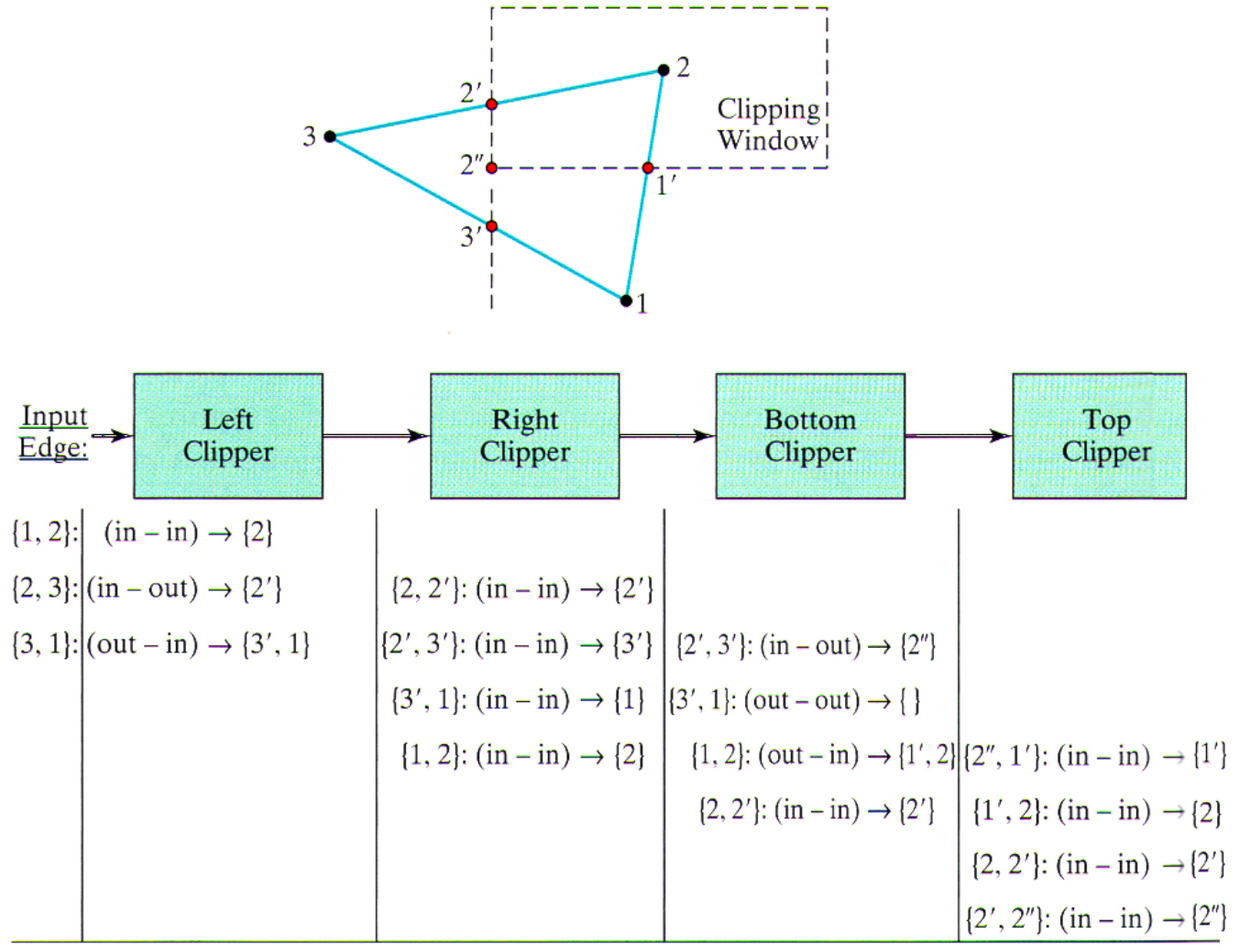
\includegraphics[width=0.7\textwidth]{Figures/RecPolAlg}
			\end{center}
	\end{figure}
\end{frame}


%%%%%%%%%%%%%%%%%%%%%%%%%%%%%%%%%%%%%%%%%%%%%%%%%%%%%%%%%%%%%%%%%%%%%%%%%%%%%%%%%%%%%%%%%%
\begin{frame}
\frametitle{Algoritmos de Recorte de Primitivas 2D}

	\begin{block}{Limitações}
		\begin{itemize}
			\item Para polígonos côncavos este algoritmo causa problemas já que ele gera apenas uma lista de vértices.
			\item Uma solução seria dividir o polígono côncavo em partes convexas.	 
		\end{itemize}
	\end{block}
	
	\begin{figure}[!h]
			\begin{center}
				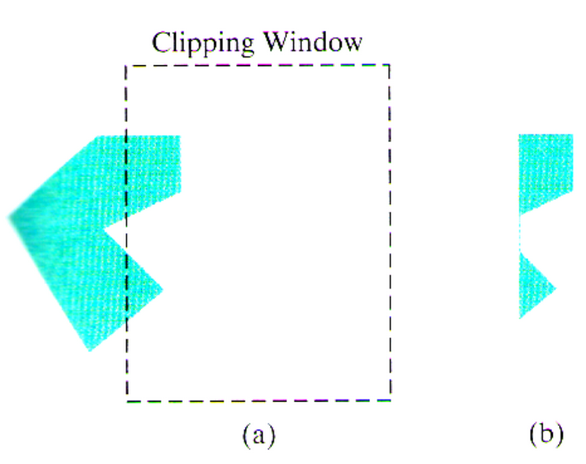
\includegraphics[width=0.4\textwidth]{Figures/PolCon}
			\end{center}
	\end{figure}
\end{frame}

%%%%%%%%%%%%%%%%%%%%%%%%%%%%%%%%%%%%%%%%%%%%%%%%%%%%%%%%%%%%%%%%%%%%%%%%%%%%%%%%%%%%%%%%%%
\subsection{Recorte de Outras Primitivas}
\begin{frame}
\frametitle{Algoritmos de Recorte de Primitivas 2D}

	\begin{block}{Recortes de Curvas}
		\begin{itemize}
			\item  As curvas podem ser recortadas com as abordagens apresentadas anteriormente.
			\begin{itemize}
				\item Se as curvas forem aproximações poligonais, é utilizado o algoritmo descrito anteriormente.
				\item Caso contrário o procedimento envolve equações não lineares.
			\end{itemize}
		\end{itemize}
	\end{block}
	
	\begin{figure}[!h]
			\begin{center}
				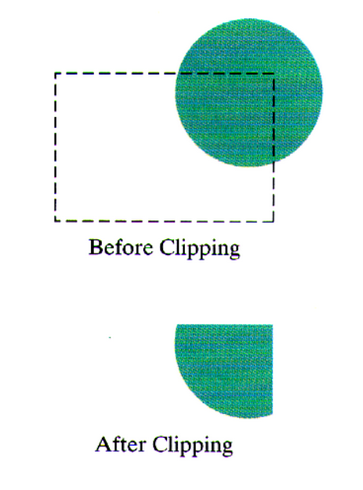
\includegraphics[width=0.3\textwidth]{Figures/RecCur}
			\end{center}
	\end{figure}
	

\end{frame}

%----------------------------------------------------------------------------------------

\end{document} 